\newaufgabe{Erklären sie warum die Berechnung von Diskrete Logarithmen und 
Quadratwurzeln in Modulararithmetik “computationally infeasible” ist, 
während in klassischer Arithmetik die entsprechenden Berechnungen 
nicht besonders aufwändig sind.}
\paragraph{Diskreter Logarithmus}
Der diskrete Logarithmus einer Zahl $m$ zur Basis $a$ modulo $p$ ist der kleinste Exponent
$x$ der Gleichung
\[
    a^x\equiv m \mod p.
\]
Das Problem bei der Berechnung ist, dass die Funktion $f(x) = a^x \mod p$ aufgrund
der Modulararithmetik nicht stetig wächst oder fällt. Die Ergebnisse für unterschiedliche
$x$ springen ohne klare Richtung. Somit kann man sich der korrekten Lösung
nicht annähern und es bleibt nur eine Brute-Force-Approach.
\begin{example}
    Sei $m = 3, p = 11$ und $a=2$.\footnote{Werte und Zahlen von \href{https://de.wikipedia.org/wiki/Diskreter_Logarithmus\#Beispiel}{Wikipedia} übernommen und nachgerechnet.}
    Man sieht in den Ergebnissen kein klar erkennbares Muster.
    \begin{figure}[h!]
        \centering
        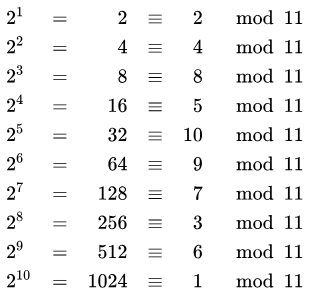
\includegraphics[width=0.4\textwidth]{img/discrete_log.png}
    \end{figure}
\end{example}
\paragraph{Quadartwurzel}
Das ziehen der Quadartwurzel bereitet im Restklassenringen mehrere Schwierigkeiten.
Eine davon ist, dass viele Zahlen überhaupt keine Wurzel besitzen.
Betrachtet man etwa den Restklassenring $\mathbb{Z}_7$ und sucht $x$, sodass
$x^2\equiv 3\mod 7$, wird man keine Lösung finden (siehe Tab \ref{ref:root_example}).
\begin{table}[htbp]
    \centering
    \begin{tabular}{c|c}
        $x$ & $x^2\mod 7$\\\hline
        0 & 0\\
        1 & 1\\
        2 & 4\\
        3 & 2\\
        4 & 2\\
        5 & 4\\
        6 & 1
    \end{tabular}
    \caption{Ergebnisse für $x^2$ in $\mathbb{Z}_7$}
    \label{ref:root_example}
\end{table}
Besonders interessant ist allerdings auch, dass sich das Ziehen der Quadartwurzel
im Restklassenring auf das Faktorisierungsproblem reduzieren lässt, welches
bekanntlich in NP liegt.